\section{Time Sensitive Networking}
\label{appendix:tsn}
An overview of the state-of-the-art research in Time Sensitive Networking (TSN) for automotive systems together with open challenges is presented in~\cite{ashjaei2021time}. It suggests the following TSN features to be implemented in new automotive networks: accurate and reliable clock synchronization (IEEE 802.1 AS) for a global, accurate and synchronized timebase, bounded latency for real-time traffic (IEEE 802.1Qav), reservation of resources for different traffic types (IEEE 802.1Qcc). To reduce jitter and achieve temporal isolation, which is necessary to achieve constructive composability as defined by~\cite{kopetz2003time}, scheduled traffic (IEEE 802.1Qbv) is needed. The work finally remarks that the Asynchronous Traffic Shaper (IEEE 802.1Qcr) is promising as it allows mixing real-time traffic types (periodic, sporadic and aperiodic) with integrated policing increasing robustness, but more research is necessary.

As mentioned in Section~\ref{sec:tsn}, according to~\cite{ashjaei2021time} the TSN standards can be grouped into four categories: Timing and synchronization, resource management, bounded low latency and finally high reliability. In the remainder of this section we summarize the main standards and group them similarly to the work presented in~\cite{ashjaei2021time}.

\paragraph{Globally accurate time base} TSN recognized that having an accurate common notion of time in a network simplifies the design and implementation of real-time systems. A globally accurate and synchronized time base is a central concept in the Time Triggered Architecture~\cite{kopetz2003time} from which TTEthernet was developed. The IEEE 802.1AS-2020~\cite{IEEE8021AS} standard specifies an algorithm called the Best Master Clock Algorithm, for determining the time reference node, called the Grand Master, in the network. The generalized precision time protocol (gPTP) takes care of synchronizing the clocks of all nodes by supplying the Grand Master clock value and taking transmission delay into account. It also provides redundancy in the clock synchronization and Grand Master clock in case of node or link failures.

\paragraph{Network resource management} In cases where real-time network traffic has a dynamic nature, e.g. an audio/video stream that only occurs at specific times in a mixed use network, TSN provides the Stream Reservation Protocol through the IEEE 802.1Qat standard~\cite{IEEE8021Qat}. The Stream Reservation Protocol reserves resources in the bridges between the source and destination nodes of the stream. Resulting in an upfront guarantee that the network meets the streams bandwidth and latency requirement. IEEE 802.1Qcc~\cite{IEEE8021Qcc} extends the Stream Reservation Protocol for more complex networks with different traffic shapers and frame preemption. While the Stream Reservation Protocol uses decentralized registration and reservation, IEEE 802.1Qcc adds centralized configuration management which can coexist with the decentralized stream reservation in the same network.

\paragraph{Deterministic transmission latency} The lack of deterministic transmission latency for Ethernet frames is caused by the network switches, called bridges in the IEEE 802.1Q-2018 standard~\cite{IEEE8021Q}. Time Sensitive Networking leverages the VLAN standard which defines eight priority classes and a strict priority scheduling algorithm. Each physical port of a bridge has a logical input and output port, when a frame enters the input port it undergoes \textit{filtering and metering} before being placed in one of eight queues that are specific for that output port. The frame's priority determines in which queue it is placed. When the output port is free to transmit a frame, the \textit{transmission selection} determines from which queue the next frame will be transmitted. As a basis TSN uses a strict priority scheduler, meaning that the queued message with the highest static priority will always be transmitted first. This can cause starvation of low priority messages.

To avoid starvation whiles still allowing prioritization an alternative \textit{transmission selection} function has been standardized: IEEE 802.1Qav~\cite{IEEE8021Qav}, known as the Credit Based Shaper (CBS). The Credit Based Shaper sits between a queue and the strict priority scheduler. Each shaper acts on one specific queue only as depicted in figure~\ref{fig:cbs}. The Credit Based Shaper limits the maximum bandwidth of a priority class by prohibiting the selection of a new frame when the allocated bandwidth has been consumed. 

The Credit Based Shaper adds fairness and smooths out traffic bursts by limiting the bandwidth of a specific traffic class, but the total delay over multiple hops can become too large for certain control applications. IEEE 802.1Qbv~\cite{IEEE8021Qbv}, called the Time Aware Shaper introduces a Stream Reservation Class \textit{CDT} for time critical data which specifies a low worst-case latency. The Time Aware Shaper uses a time-division multiple access scheme to define a cyclic network schedule called the \textit{gate control list}. The schedule splits the network bandwidth up into time slices and defines which of the Ethernet priorities are allowed to transmit during that time slice. A gate between the queue output and the priority scheduler entry opens or closes to allow or block frames to be selected by the scheduler. The Time Aware Shaper can be used to avoid large buffering effects in the switches and removes non-deterministic interruptions by non-real time traffic.

\begin{figure}[htbp]
    \centering
    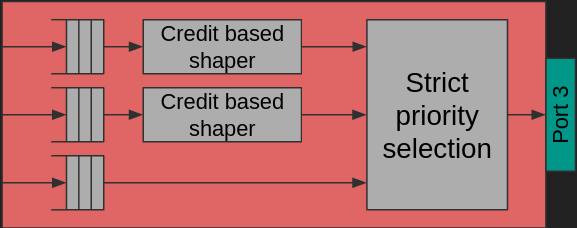
\includegraphics[width=0.6\textwidth]{images/cbs.png}
    \caption{An output port with three queues and the transmission selection implementation consisting of two credit based shapers and a strict priority scheduler}
    \label{fig:cbs}
\end{figure}

Other shapers exist such as the IEEE 802.1Qcr~\cite{IEEE8021Qcr} Asynchronous Traffic Shaper and IEEE 802.1Qch~\cite{IEEE8021Qch} Cyclic Queuing and Forwarding standards. Each working differently and solving a specific problem. The last relevant standards for bounded low latency are the related standards IEEE 802.3br~\cite{IEEE8023br} and IEEE 802.1 Qbu~\cite{IEEE8021Qbu} which together allow lower priority frames to be preempted during their transmission. The smallest transmittable chunk is still 64 bytes, so higher priority frames will still experience some delay. \todo{preemption buffer na de gate, waardoor je preempted bericht alsnog delay kan veroorzaken op een later moment terwijl zijn gate al gesloten is.}

\paragraph{Reliable frame transmission} In certain applications it is critical that messages are received without errors in their content. Ethernet protects the frame data by appending a cyclic redundancy check and requiring a frame to be dropped when the CRC does not match the received data. Other reasons that a frame is not received can be: switch queues overflowing and hardware failure of connectors or cables. The IEEE 802.1CB Frame Replication and Elimination for Reliability~\cite{IEEE8021CB} (FRER) standard duplicates frames and sends them over multiple disjoint paths to increase the chance that a frame arrives at the destination. The first duplicate which arrives at the destination and passes the CRC check is considered correct, the remaining frames will be discarded upon reception. If a node does not implement FRER the closes FRER aware switch will transparently duplicate/eliminate the frames. In an automotive setting one could imagine two disjoint paths on either side of the vehicle to increase the reliability of the network by placing the redundant paths physically far apart.

\paragraph{}In conclusion there is not one type of Time Sensitive Network, TSN is a set of different standards trying to solve different problems in multiple ways. Depending on the requirements several standards can be combined to create an Ethernet based network that is capable of reliable, time deterministic and low latency transmission of Ethernet frames. For example the Credit Based Shaper can be combined with the Time Aware Shaper to mix hard, soft and non-real time traffic in a single network. Combined with Frame Replication and Elimination to reliably and transparently deliver the frames over two disjoint paths.
